\documentclass[uplatex]{jsarticle}
\usepackage[top=20truemm, bottom=20truemm, left=20truemm, right=20truemm]{geometry}
\usepackage{url}
\usepackage{booktabs}
\usepackage{here}
\usepackage{amsmath, amssymb}
\usepackage[dvipdfmx]{graphicx}

% 表の中でもfootnoteを使えるように
\usepackage{footnote}

\title{
    \vspace{-1.5cm}
    サイバーセキュリティ Assignment 3 \\
    Incident 1
}
\author{group 6}

\begin{document}
\maketitle

\subsubsection*{担当者}
\begin{table}[H]
    \begin{tabular}{|c|l|l|}
        \hline
        学生番号 & 氏名 & 所属研究室\\
        \hline\hline
        1911403 & 佐々木 皓大 & ユビキタスコンピューティングシステム研究室\\
        \hline
        2011067 & 奥村 嶺 & 情報基盤システム学研究室(Inet-Lab)\\
        \hline
        2011115 & 佐伯 雄飛 & \\
        \hline
    \end{tabular}
\end{table}

\section*{Step 1}
\subsection*{Q}
For each incident, provide a detailed summary of the incident report toward cybersecurity professionals, by fully mobilizing concepts that you learned through these lectures. Create a timeline of the incident, as well as a fishbone diagram, that illustrates root cause and other important events in order to help with the understanding.
\subsection*{A}
我々は 2017年3月に発生した,
B.LEAGUEチケットサイトとファンクラブ受付サイトへの不正アクセスによる
個人情報流出インシデント
\footnote{
    ぴあ社がプラットフォームを提供するB.LEAGUE チケットサイト,及びファンクラブ受付サイトへの不正アクセスによる,個人情報流出に関するお詫びとご報告
    : \url{https://corporate.pia.jp/news/files/security_incident20170425.pdf}
}
について調査した.
まず,インシデント発生時の状況を述べる.
B.LEAGUE(国内男子プロバスケットボールリーグ)はチケットサイトとファンクラブ受付サイトの運営を,
ぴあ株式会社(以下ぴあ社と表記)に委託していた.
また,受託したぴあ社は実際のサイトの開設と運用を外部の会社
(チケットサイトはH社,ファンクラブ受付サイトはK社)に発注していた.
H社とK社では,サイトの構築フレームワークとして,
The Apache Software Foundationが管理しているApache Struts2
\footnote{
    Welcome to the Apache Struts project
    : \url{https://struts.apache.org/}
}
を用いていた.
悪意ある攻撃者は,このApache Struts2に含まれる脆弱性を用いて,
Webサーバー及びデータベースサーバへの不正アクセスし,
最大約15万5千件の個人情報を入手した
\footnote{
    B.LEAGUE チケットサイト及びファンクラブ受付サイトにおける個人情報流出事案に関する,その後のお詫びとご報告
    : \url{https://corporate.pia.jp/news/files/security_incident20170518.pdf}
}
とされている.
次に,インシデント発生時のタイムラインを表\ref{tab:incident_timeline}に,
特性要因図 (fish bone diagram) を図\ref{fig:fishbone}に示す.

% !TeX root = ./main.tex

\begin{savenotes}
\begin{table}[htbp]
    \centering
    \caption{インシデントタイムライン}
    \label{tab:incident_timeline}
    \begin{tabular}{|l|p{8cm}|}
    \hline
    2017年3月6日 & Apache Struts 2 に関する脆弱性 S2-045 が Wiki\footnote{
        S2-045 - Apache Struts 2 Wiki - Apache Software Foundation
        : \url{https://cwiki.apache.org/confluence/pages/viewpage.action?pageId=68717772}
    }
    に投稿される(3/2にV1が出ているが,バージョン 2.3.32 について言及されておらず不完全と判断した) \\ \hline
    2017年3月7日 & Github で攻撃コード公開\footnote{
        xsscx氏による一例: \url{https://github.com/xsscx/cve-2017-5638}
    } \\ \hline
    2017年3月9日 & IPAが管理する,Apache Struts2の脆弱性対策情報一覧ページ
    \footnote{
        Apache Struts2 の脆弱性対策情報一覧
        : \url{https://www.ipa.go.jp/security/announce/struts2_list.html}
    }
    に S2-045 が追加される \\ \hline
    2017年3月10日 & ぴあ社が S2-045を社内で認識する \\ \hline
    2017年3月7日~15日(後の検証で判明) & ぴあ社が運営するECコンテンツ「B.LEAGUE チケットサイト,及びファンクラブ受付サイト」が何者かにサイバー攻撃を受ける.(IPAの発表によりApache Struts2の脆弱性をぴあ社内で認識していたが,webサーバ上にクレジット情報は保存されてないと認識していた) \\ \hline
    2017年3月17日 & SNSサイト「Twitter」にて,クレジットカードの不正利用に関する書き込みが続出.クレジットカード会社より,不正利用の形跡があると報告を受ける. \\ \hline
    2017年3月25日 & ぴあ社は,当該ウェブサイト上でのクレジットカード決済機能を停止.同時に第三者調査機関に調査を依頼する. \\ \hline
    2017年4月25日 & ウェブサイト上にて,不正アクセス被害の報告と謝罪を実施.予想される被害総数は15万4,599件(うちカード関係の情報は3万2,187件)と発表. \\ \hline
    2017年4月28日 & 同社CCOを委員長とする再発防止委員会を組成.再発防止に向けて取り組む. \\ \hline
    2017年5月18日 & 第三者調査機関の報告を受けて,ウェブサイト上で続報を発表.既に公表されていたカード情報3万2,187件とは別に,新たに6,508件の漏えいの可能性があることを公開. \\ \hline
    \end{tabular}
\end{table}
\end{savenotes}


\begin{figure}[htbp]
    \centering
    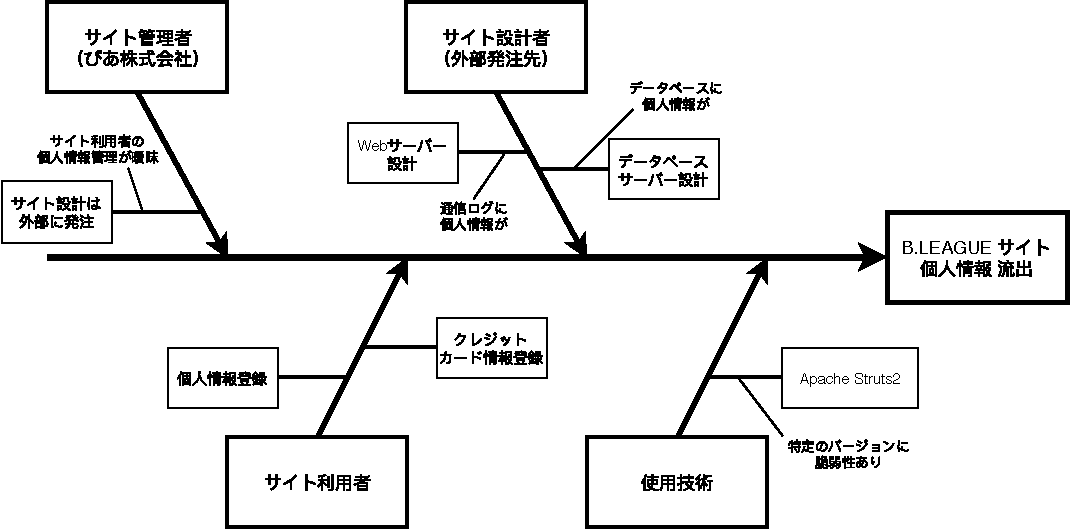
\includegraphics[width=0.8\linewidth]{pic/fishbone-GroupA.pdf}
    \caption{特性要因図}
    \label{fig:fishbone}
\end{figure}

\section*{Step 2}
\subsection*{Q}
Identify technical factors that led to each incident. Based on the real timeline of the particular incident, identify two critical periods where technical intervention was necessary.
\subsection*{A}
インシデント対応に重要とされる技術的要因については,
サイトのフレームワークとしてApache Struts2を用いていたことが挙げられる.
Step 1にも記述した通り,
ぴあ社が運営していたサイトの基盤部分には Apache Struts2 が使用されており,
攻撃者は脆弱性 S2-045 を利用しサイトがホストされているサーバを不正に操作したとされている.
ここで,脆弱性 S2-045 の概要について示す.この脆弱性は,ファイルアップロード時に,
Apache Struts 2にてデフォルトで使用される,マルチパーサー「jakarta」に起因する.
ファイルアップロードの実行中に例外処理とエラーメッセージの生成に誤りがあり,
リモートの攻撃者が細工したContent-Type,Content-Disposition,
またはContent-Length HTTPヘッダを介して任意のコマンドを実行することを可能にしている.
S2-045のCVEコードはCVE-2017-5638であり,CVSS 2.0 : 10.0 HIGH (AV:N/AC:L/Au:N/C:C/I:C/A:C),
CWE-20 : Improper Input Validation と分類
\footnote{
    NVD - CVE-2017-5638
    : \url{https://nvd.nist.gov/vuln/detail/CVE-2017-5638}
}
されている.一般的な脆弱性の影響として表\ref{tab:influence}に示す.
今回のケースでは機密性に影響を与える可能性が考えられる.
よって機密データの管理状態を確認する必要性がある.
次に,技術的に介入が必要とされた時期について述べる.
表\ref{tab:incident_timeline}より,
2017年3月6日にApache Struts2 の脆弱性であるS2-045(CVE-2017-5638)が報告されている.
しかしぴあ社は10日にこの脆弱性を認識している.
この4日間の時間誤差がインシデントを招く要因のひとつと考えられ,
6日に技術的介入が必要であると考えられる.
具体的に6日時点ではまだパッチファイル等は公開されていないため,
使用範囲の認識やマルチパーサーの停止,別のマルチパーサーへ切り替えを議論する必要があると考える.
また,SBテクノロジー株式会社が公表しているCVE-2017-5638 - 脆弱性調査レポート
\footnote{
    CVE-2017-5638 - 脆弱性調査レポート
    : \url{https://www.softbanktech.co.jp/special/cve/2017/0004/}
}
によると,
2017年3月8日時点でApache Software Foundation より,
この脆弱性を修正するバージョンがリリースされている.
この脆弱性が修正されたバージョンへとアップグレードすることを推奨し,
ただちにアップグレードすることが困難である場合,「Content-Type」のバリデーションを行い,
”multipart/form-data”と一致しないリクエストを破棄する
サーブレットフィルターを実装することにより問題を回避することが可能である.
この日にアップグレードするもしくはバリデーションを行う等の介入を進めることも必要と考えられる.
よって介入時期として2017年3月6日および2017年3月8日とする.

\begin{table}[htbp]
    \centering
    \caption{影響範囲と内容}
    \label{tab:influence}
    \begin{tabular}{|c|p{10cm}|}
    \hline
    影響範囲 & 影響内容 \\ \hline
    可用性 & 予期しない値の入力により,プログラムがクラッシュ,あるいはメモリや CPU 等のリソースを過度に消費する可能性がある. \\ \hline
    機密性 & 攻撃者がリソースの参照を制御可能な場合,機密データを読み取る可能性がある. \\ \hline
    完全性 & 任意のコマンド実行を含めた悪意ある入力により,予期しない方法でデータや制御フローを改ざんされる可能性がある. \\ \hline
    \end{tabular}
\end{table}

\section*{Step 3}
\subsection*{Q}
Identify human factors that led to each incident. Based on the real situation of the particular incident, describe how best you would deliver risk messages, as an external security consultant, in the two critical periods that you identified in the step 2.
\subsection*{A}
まず人為的要因としては,以下の3項目が考えられる.
\begin{itemize}
    \item サービス管理者(ぴあ社)
    \item サービス開発者(ぴあ社の外注先会社)
    \item 悪意あるユーザ
\end{itemize}
各項目について概要を示す.
サービス管理者において,前述のとおり,
サイトを構築するためのフレームワーク「Struts2」の脆弱性はたびたび報告されていた.
しかし,報告資料によると,
ぴあ社はこの脆弱性については事故直前の3月10日にIPAの発表で初めて把握したとしている.
初動調査においてもこの脆弱性が考慮されていなかった可能性が高いと考えられる.
その結果,クレジットカード会社から連絡を受けるまで,
サイトユーザに対して特にケアは行わなかったことで,被害が拡大してしまった可能性がある.
サイト製作を委託発注していたとしているが,この状況より,
完全に任せきりになっていたのではないかと思われる.
システムの脆弱性など,リスク要因になるものについては,
できる限り早い段階から情報収集し,関係者と共有しておくのが望ましい.
ぴあ社の個人情報管理の仕組み・体制に問題があったと言えるだろう.
サービス開発者において,ぴあ社の外注先会社がサイトユーザの個人情報の取り扱いに関して,
運用ガイドラインと異なる不適切な管理を行っていたこと,
および,ぴあ社がそれを認知していなかったことが挙げられる.
ぴあ社からの発表によると,運用ガイドライン上では,
サイトを利用するユーザの個人情報は外注先のH社とK社のWebサーバや
データベース上に残さないとされていた.
しかし,情報漏えいが発覚した当初では,
クレジットカード情報を含む個人情報が,
H社の通信ログ上とK社のデータベース上に保持されていた事実がある.
これらは,結果として個人情報流出を助長する1要因となったとされている.
悪意あるユーザにおいては,Apache Struts2 に対する脆弱性が3/6に公開された後,
3/7にGithubに攻撃コード(PoC)が公開された.
その結果,彼らはより迅速に攻撃行動に移ることが可能となり,被害が拡大したと考えられる.

\end{document}
